\documentclass[11pt,twoside,a4paper]{article}
\usepackage{amssymb}
\usepackage{amsmath}
\usepackage{graphicx}
\usepackage{float}
% \usepackage[usenames,dvipsnames]{pstricks}
% \usepackage{epsfig}
% \usepackage{pst-grad} % For gradients
% \usepackage{pst-plot} % For axes
% \usepackage[space]{grffile} % For spaces in paths
% \usepackage{etoolbox} % For spaces in paths


\begin{document}
\title{Adversarial examples}
\maketitle

\section{Problem formumation}
Given an image
$\textbf{I}_{i,j,k} := \{i, j, k\; |\; 0\le i, j, k\le 255\} \in
\mathbb{R}^{m \times n \times 3}$ an adversary with malicious intentions can
construct a malformed copy of $I$, which we will call
$I^{\left( p \right)}$, by modifying its pixel values. Usually these
attacks consists of adding small perturbations of $\left(+/-1\right)$
bit of information into the pixel values and have a twofold
goal. First, to deceive any human evaluator since they are
imperceptible by the human eye. Second, to expoit the predictive
system in favour of the adversary by intentionally manipulating the
outcome of the prediction, thus, one can say that they pose a security
risk to prediction systems including but not limited to, deep neural
networks (DNNs). We proceed by explaining two of the most well know
perturbation attacks which will be used as a comparision metric to
measure the robustness of our approach during the experiments. The
first of the methods presented was proposed by [citation]. It exploits
the gradients of the loss function
$\epsilon \cdot \mbox{sign}\left( \nabla_{x}J\left( \textbf{I}, y \right) \right)$ with
respect to the input $\textbf{I}$, where the loss is defined as

\begin{align}
  J\left( \textbf{I}, y \right) :=& -\frac{1}{N}\left[
                                    \sum_{n=1}^{N}\sum_{c=1}^{C} y_{c}^{\left( n \right)}\log\left(
                                    \hat{y}_{c}^{\left( n \right)} \right) + \left( 1 - y_{c}^{\left( n
                                    \right)} \log\left( 1 - \hat{y}_{c}^{\left( n \right)} \right)
                                    \right) \right] + R(\bf{\Omega})
                                  & \\
  R\left( \bf{\Omega} \right) =&
                            -\frac{\lambda}{2N}\sum_{l=1}^{L-1}\sum_{i=1}^{U_{l}}\sum_{j=1}^{U_{l+1}}
                            {\left( \textbf{W}_{ij}^{\left( l \right)}
                            \right)}^{2}
\end{align}

$n = \{1,\ldots, N\}$ denotes the number of training samples

$c = \{1,\ldots, C\}$ denotes the number of classes

$y_{c}^{\left( n \right)}$ is the true label for class $c$ of the
training sample $n$

$\hat{y}_{c}^{\left( n \right)}$ equivalently is the predicted one

$l = \{1,\ldots, L-1\}$ denotes the number of layers in the network

$i = \{1,\ldots,U_{l}\}$ denotes the number of units/nodes for layer $l$
and $l+1$ equivalently.

The intuition is that we want to maximize an $\epsilon$ which emphasizes the
pixels in the picture that the neural network thinks is important. In
other words we want to maximize the dot product in the direction we're
moving $\epsilon$ and the gradient. The second method proposed by
[citation] is split in two folds. First, estimation of the direction
of sensitivity of the network with respect to the input
$\textbf{I}$. Second, selecting the appropriate perturbation. The
direction sensitivity step evaluates the sensitivity of class change
to each input feature while the perturbation selection uses the
sensitivity information to select a perturbation
$\epsilon\cdot\textbf{I}$ among the input dimensions. In other words the goal is
to find the dimensions of $\textbf{I}$ that will produce the expected
adversarial behaviour with the smallest perturbation. One can achieve
that by evaluating the sensitivity of the network to changes to the
input components of $\textbf{I}$. In this method the Jacobian of the
network is exploited to compute gradients of the output components
with respect to each input in order to define the sensitivity of the
network for a given input $\textbf{I}$ in each of its dimensions.

\section{Hypothesis proposal}

The goal is given a baseline deep neural network model $M_{0}$, which
outputs a probability indicating the confidence in the predicted class
with respect to the input image $\textbf{I}$, to reduce its
sensitivity against adversarialy perturbed inputs
$I^{\left( p \right)}$. One way to achieve this is to use an
additional constraint in the loss function to penalize the gradients
of the input images $\textbf{I}$ that lead to adversrial perturbations
but this would also have an impact on the generalization of the
network. An alternative approach would be to incorporate 2 additional
models $M_{1}$ and $M_{2}$ where one of them is a generative model and the
other is a regular descriminative network. In summary, we have a
totatl of 3 models $\{M_{0}, M_{1}, M_{2}\}$ out of which only one is a
generative model. Given an input image $\textbf{I}$ we feed it through
at the same time to 2 of the models, $M_{0}$ which is a discriminative
model and $M_{1}$ which is a generative model. $M_{0}$ outputs a
prediction vector $\vec{y} \in \mathbb{R}^{c}$ with values in the range
[0,1] while $M_{1}$ outputs an image
$I^{\left( g \right)} \in \mathbb{R}^{m \times n \times 3}$. We now
take both $\left( \textbf{I}^{\left( g \right)}, \vec{y} \right)$ and
use them as input into our 3rd model $M_{3}$ for the final
classification, where $\textbf{I}^{\left( g \right)}$ operates as the
input data while $\vec{y}$ operates as the labels. The intuition is
that everytime that there's an adversarial image
$\textbf{I}^{\left( p \right)}$ it's going to be a discrepancy between
the outputs of model $M_{0}$ and $M_{1}$ which in turn will cause a
reduction in the final classification accuracy of the model $M_{3}$. Some
of the problems in regards to the generative models is the fact that
sometimes it generates samples whihc are not close to the original
images due to the large variety of classes in the dataset.

\begin{figure}[H]
  \centering
  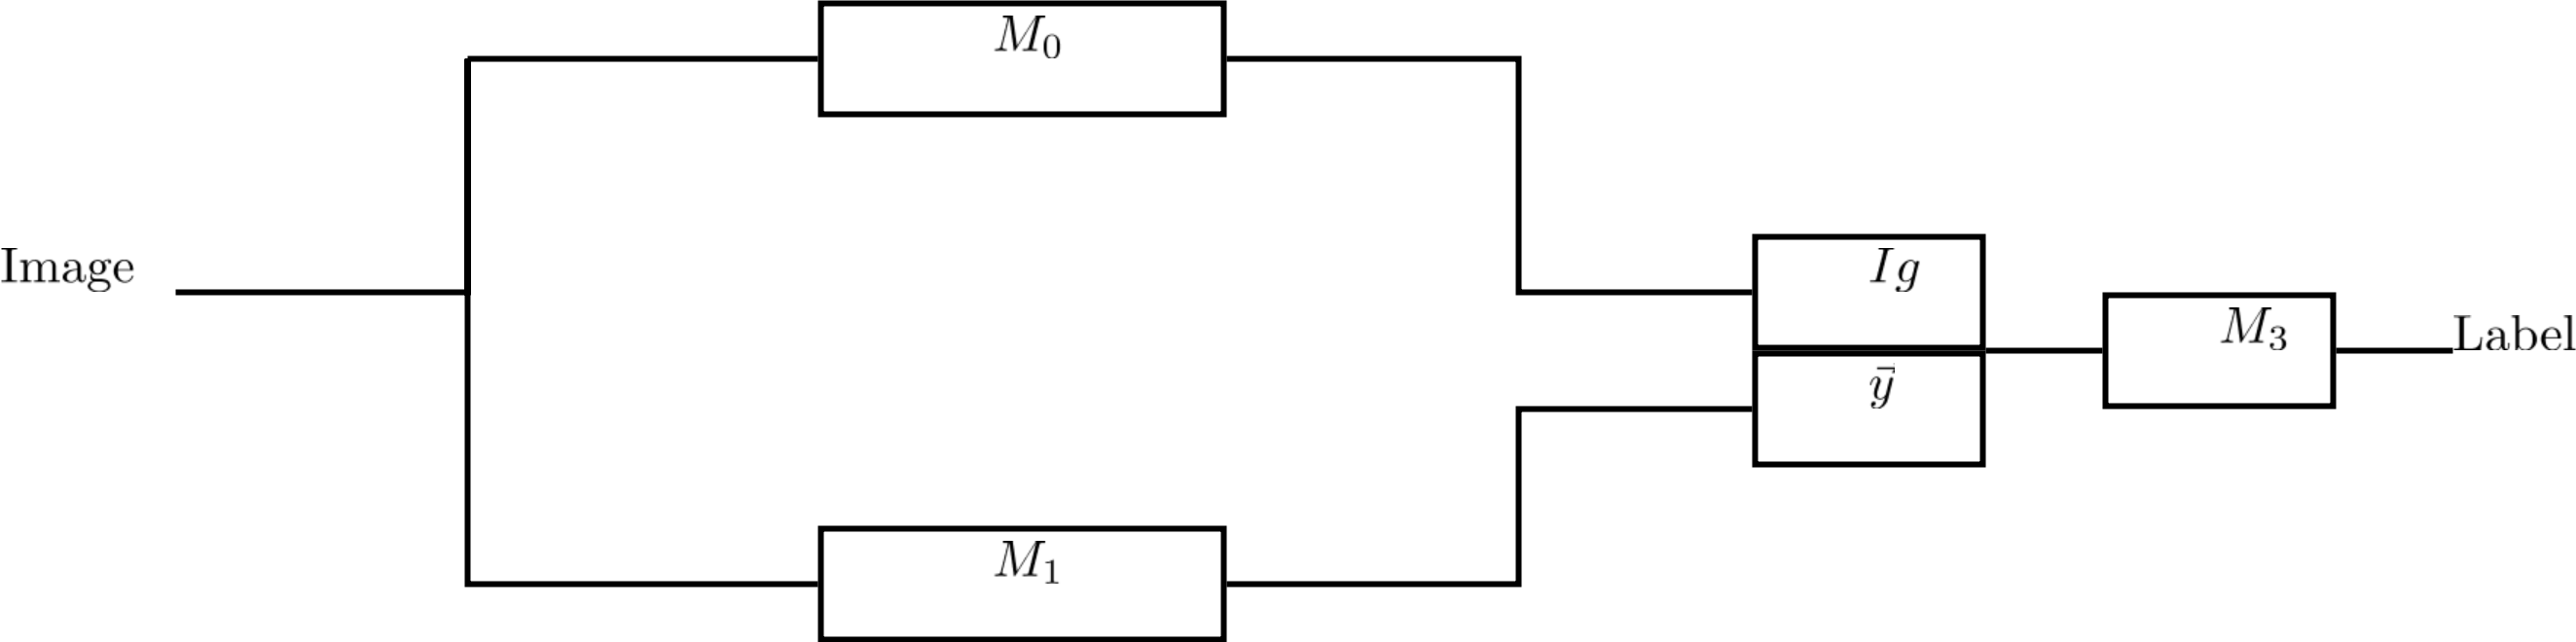
\includegraphics[width=\linewidth]{schema}
  \caption{Schema of proposed model.}
\end{figure}



\end{document}


%%% Local Variables:
%%% mode: latex
%%% TeX-master: t
%%% End:
